\documentclass[10pt,twocolumn,letterpaper]{article}
\usepackage{cvpr}
\usepackage{times}
\usepackage{epsfig}
\usepackage{amsmath}
\usepackage{amssymb}
\usepackage{booktabs} % for much better looking tables
\usepackage{array} % for better arrays (eg matrices) in maths
\usepackage{paralist} % very flexible & customisable lists (eg. enumerate/itemize, etc.)
\usepackage{verbatim} % adds environment for commenting out blocks of text & for better verbatim
\usepackage{subfigure} % make it possible to include more than one captioned figure/table in a single float
\usepackage{graphicx}
\usepackage{multirow}
% Include other packages here, before hyperref.
% If you comment hyperref and then uncomment it, you should delete
% egpaper.aux before re-running latex.  (Or just hit 'q' on the first latex
% run, let it finish, and you should be clear).
%\usepackage[pagebackref=true,breaklinks=true,letterpaper=true,colorlinks,bookmarks=false]{hyperref}
\cvprfinalcopy % *** Uncomment this line for the final submission
\def\cvprPaperID{****} % *** Enter the CVPR Paper ID here
\def\httilde{\mbox{\tt\raisebox{-.5ex}{\symbol{126}}}}
% Pages are numbered in submission mode, and unnumbered in camera-ready
\ifcvprfinal\pagestyle{empty}\fi
%use \x, \y, and \w for bold vector forms
\newcommand{\x}{\bold{x}}
\newcommand{\xb}{\bar{x}}
\newcommand{\y}{\bold{y}}
\newcommand{\yb}{\hat{y}}
\newcommand{\w}{\mathbf{w}}
\DeclareMathOperator*{\argmax}{arg\,max}
\begin{document}
%%%%%%%%% TITLE
\title{
Project in CSE 250B\\
Assignment 3: Conditional Random Fields}
\author{Andreas Landstad, Spencer Bliven, Jonas Hoelzler\\
Computer Science Department\\
University of California, San Diego\\
{\tt\small landstad.andreas@gmail.com, sbliven@ucsd.edu, jonas@hoelzler.de}
}% For a paper whose authors are all at the same institution,
% omit the following lines up until the closing ``}''.
% Additional authors and addresses can be added with ``\and'',
% just like the second author.
% To save space, use either the email address or home page, not both
%\and
%Second Author\\
%Institution2\\
%First line of institution2 address\\
%{\tt\small secondauthor@i2.org}
\maketitle
\thispagestyle{empty}
%%%%%%%%% ABSTRACT
\begin{abstract}

As result we obtained 74\% word accuracy and about 96\% letter level accuracy.
\end{abstract}
%%%%%%%%% BODY TEXT
%INDICES:
% words n=1...N
% features j=1...J
% positions i=1...M_n
% tags k=1...V
%LABELS
% y_n is the correct label
% y' is any label
% \hat{y} is the predicted label
% tags are u or v
% problem: y_1 is ambiguous: i=1 or n=1?
% \xb aka \hat{x} is a vector of letters


\section{Introduction}

Conditional random fields provide a generic model for performing supervised learning. Generic feature functions are used to transform complicated input data and labels into real numbers. This abstraction allows machine learning and statistical analysis on very complicated datasets.

One problem for which this is useful is automatic detection of syllable boundaries within words. Possible inputs include all words in a given language, plus the possibility of additional  neologisms which may be coined after the training period. Developing a classifier to determine syllable boundaries is an important task for automatic hyphenation, speech synthesis, and linguistic analysis.


\subsection{Conditional Random Field model}
The goal of supervised classification is to predict a label, $\y$, from some input data, $\x$. Conditional random fields do not place any restrictions on the type of data and labels being learned. To allow this abstraction, conditional random fields introduces the concept of \begin{em}feature functions\end{em} of the form $F(\x,\y)$ which attempt to measure the compatibility of $\x$ with the label $\y$. A number of such feature functions are calculated for each $(\x,\y)$ pair, and the weighted sum of $J$ feature functions is used to determine the probability that $\y$ is the correct label for $\x$, according the the equation
\begin{equation}
       p(\y\,|\,\x;\w) = \frac{\exp \left( \sum_{j=1}^J w_j F_j (\x,\y) \right)}{z(\x;\w)}
\end{equation}
where $z(\x;\w)$ normalizes the total mass over all possible labels $y'$ to one and is equal to
\begin{equation}
       z(\x;\w) = \sum_{\y'} \exp \left( \sum_{j=1}^J w_j F_j (\x,\y) \right). \label{Eq:partition}
\end{equation}

To use this model for inference, one simply assigns the most probable label for a given $\x$,
\begin{align}
       \hat{y} & =\argmax_{\y} \, p(\y\,|\,\x;\w) \\
               &= \argmax_{\y} \sum_{j=1}^J w_j F_j(\x,\y).
               \label{equation}
\end{align}

The weights vector $\w$ is learned according to the principle of maximum likelihood. Thus, for some set of training pairs $(\x_n,\y_n)$ for $n=\left\{1,2,\dots,N\right\}$, the objective function is to maximize the total log likelihood with respect to $\w$ over all points of
\begin{align}
       LCL(\w) &= \sum_{n=1}^N \log\,p(\y_n\,|\,\x_n ;\,\w) \\
               &= \sum_{n=1}^N \left( \sum_{j=1}^J w_j F_j (\x_n,\y_n) - \log z(\x_n;\w) \right).
\end{align}

During training, $L_2$ regularization is used such that most weights are near zero. This is important to prevent overfitting, since the number of features is often greater than the number of training pairs, resulting in an underspecified system. The regularized objective is
\begin{align}
       LCL^*(\w) &= \sum_{n=1}^N \log\,p(\y_n\,|\,\x_n ;\,\w) - \lambda N\parallel \w \parallel^2 \\
               &= \sum_{n=1}^N \left( \sum_{j=1}^J w_j F_j (\x_n,\y_n)  - \log z(\x_n;\w) \right) \notag \\
               &\hspace{1 em}  - \lambda N\parallel \w \parallel^2
               \label{Eq:rLCL}
\end{align}
where $\lambda$ is the strength of regularization.


\subsection{Linear Chain CRFs}

Training a CRF means finding the weight vector w that gives the best possible prediction for equation (\ref{equation}) for each training example $\x$. For the general case, computing Eq. \ref{equation} takes exponential time to iterate over all possible values.

This problem can be circumvented by restricting the model to linear chain CRFs. This refers to CRFs with features which depend only on two consutive tags. This allows all features $F_j(\x,\y)$ to be decomposed into low-level feature functions
\begin{align}
F_j(\x,\y) &= \sum_{i=1}^{M_n} f_j(y_{i-1},y_{i},\x,i).
\end{align}

For linear chain CRFs, Eq \ref{equation} can be computated efficiently by the Viterbi algorithm.
The $g_i$ values are assumed to be given by preprocessing as a $m$ by $m$ Matrix:
\begin{align}
g_i(y_{i-1},y_i) = \sum_{j=1}^{J} w_j f_j(y_{i-1},y_{i},x,i))  
\end{align}
Let $v$ range over the range of tags. Define $U(k, v)$ to be the score of the best
sequence of tags from position $1$ to position $k$, where tag number $k$ is required to
equal $v$. This is a maximization over $k - 1$ tags because tag number k is fixed to
have value v. Formally,
\begin{align}
U(k,v)=max_{y_1 .. y_k} \sum_{i=1}^{k-1} g_i(y_{i-1},y_i) + g_i(y_{i-1},v)
\end{align}
which can be implemented efficiently recursive as
\begin{align}
U(k, v) = max_u [U(k-1, u) + g_k(u, v)]
\label{recu}
\end{align}
Now, one can backtrack the path, which gives the highest probability.
\subsection{Training via Stochastic Gradient Ascent}
The weight vector $\w$ that maximizes Equation \ref{Eq:rLCL} can be found using gradient ascent methods. The gradient of the $LCL$ with respect to the $j$th component of $\w$ is
\begin{align}
       \frac{\partial LCL^*}{\partial \w_j } &=
               \sum_{n=1}^N \frac{\partial}{\partial \w_j }  \log\,p(y_n\,|\,\x_n ;\,\w)  \notag \\
       &\hspace{1 em} - \lambda N  \frac{\partial}{\partial \w_j }\parallel \w \parallel^2 \\
       %&= \sum_{n=1}^N \left( F_j(\x_n,y_n) -  \sum_{\y'} p(\y'\,|\,\x_n ;\,\w)\,F_j(\x_n, \y' ) \right)  \notag \\
       %&\hspace{1 em}         - 2 \lambda N   \w_j \\
       &= \sum_{n=1}^N \left( F_j(\x_n,y_n) -   \mathbb{E}_{\y'\,|\,\x_n} \left[ F_j(\x_n, \y' ) \right] \right)  \notag \\
       &\hspace{1 em}         - 2 \lambda N   \w_{j}. \label{Eq:gradient}
\end{align}
The expectation in equation \ref{Eq:gradient} can be calculated by summing over all possible labels $\y'$ according to
\begin{align}
       \mathbb{E}_{\y'\,|\,\x_n} \left[ F_j(\x_n, \y' ) \right] &= \sum_{\y'} p(\y'\,|\,\x_n ;\,\w)\,F_j(\x_n, \y' ). \label{Eq:expectation}
\end{align}
% Define \M for forwards-backwards score
\newcommand{\M}{\mathcal{M}}
For general CRFs computing the expectation is computationally intensive since it requires summing over $V^M_n$ possible length-$M_n$ labels. For linear chain CRFs this can be solved in time $O(M_n V^2 J^2 + V^2 M_n)$ using the
\begin{em}forwards-backwards\end{em}
algorithm, which is large but polynomial. The forwards-backwards algorithm involves computing two functions recursively. Let $\alpha(i,u)$ be the unnormalized  probability of the tag sequence $y_1 y_2 \dots y_i$ ending with $y_i  = u$. This can be calculated as
\begin{align}
       \alpha(i,u) &= \sum_{k=1}^V \alpha(i-1, v_k) \M_i(v_k,u)
\end{align}
for all tags $v_k$, where $\M_i(v_k,u)$ is the score
\begin{align}
       \M_i(v,u) &= \exp \sum_{j=1}^J w_j\, f_j(v,u,\x,i).
\end{align}
The base case for the forwards vector is
\begin{align}
       \alpha(1,v) = \M_i(\mbox{\textsc{begin}},v)
\end{align}
The backwards vector, $\beta(u,i)$, is the unnormalized probability of the tag sequence $\y_i \y_{i+1}\dots \y_{M}$.  This is given as
\begin{align}
       \beta(u,i) = \sum_{k=1}^V \beta(v_k,i+1)\M_{i+1}(u,v_k)
\end{align}
with base case
\begin{align}
       \beta(v,n) = \M_{i+1}(u,\mbox{\textsc{end}}).
\end{align}
Together, the forwards and backwards algorithm can be used to calculate the partition function (Eq.\ \ref{Eq:partition}) and conditional expectation (Eq.\ \ref{Eq:expectation}).
\begin{align}
       z(\x_n;\w) &= \sum_{k=1}^V \alpha(M_n, v_k) \M_{M_n}(v_k,\mbox{\textsc{end}}) \\
       &= \sum_{k=1}^V \beta(v_k, 1)  \M_1(\mbox{\textsc{begin}}, v_k)
\end{align}
\begin{align}
       p(y_i = u | \x; \w) &= \frac{\alpha(i,u)\beta(u,i)}{z(\x;\w)}
\end{align}
\begin{align}
       p(y_{i-1}=u,y_i=v|\x;\w) &= \frac{\alpha(i,u)\M_{i+1}\beta(v,i+1)}{z(\x;\w)}
\end{align}
\begin{align}
       \mathbb{E}_{\y'\,|\,\x_n} & \left[ F_j(\x_n, \y' ) \right]
               = \sum_{i=1}^{M_n} \mathbb{E}_{\y'\,|\,\x_n} \left[f_j(y_{i-1},y_i,\x_n, i ) \right] \\
               &= \sum_{i=1}^{M_n} \sum_{k=1}^V \sum_{l=1}^V \big[ p(y_{i-1}=v_k,y_i=v_l\,|\,\x_n ;\,\w) \notag \\
               & \hspace{6 em} \cdot f_j(y_{i-1},y_i,\x_n, i ) \big] \\
               &= \sum_{i=1}^{M_n} \sum_{k=1}^V \sum_{l=1}^V \Big[ f_j(y_{i-1},y_i,\x_n, i ) \notag \\
               & \hspace{6 em} \cdot  \frac{\alpha(i,u)\M_{i+1}\beta(v,i+1)}{z(\x;\w)} \Big]
\end{align}

Using the forwards-backwards algorithm to calculate the gradient of $LCL*$, standard stochastic gradient ascent can be used to find the maximum $\w$ with the update rule
\begin{align}
    w_j \leftarrow w_j + \lambda \frac{\partial}{\partial w_j} LCL^*(y_n|\x_n; \w)
\end{align}
for each training pair $n=1,2,\ldots,N$.


\subsection{Collin's Perceptron Algorithm}
Although the forwards-backwards algorithm allows the computation of the gradient in polynomial time, this is still a significant computational challenge. Collin�s Perceptron Algorithm attempts to improve on that time by approximating the gradient.

By placing all the probability mass on the most likely $\y$ value, i.~e.~by using the approximation $p(\y|\x;w) = I(y = \hat{y})$, where $\hat{y}=argmax_y p(\y|\x;w)$,
the stochastic gradient update rule simplifies to
\begin{align}
       w_j := w_j + F_j(\x, \y)
       w_j := w_j . F_j(\x, \hat{y}).
\end{align}
This rule is applied for every weight $w_j$, for a given training example $\langle x, yi\rangle$. Given
a training example $\x$, the label $\hat{y}$ can be thought of as an impostor compared to the true label y \ref{elkan}.


\section{Methods}

\subsection{Zulu Dataset}
The Zulu dataset consists of 10,040 Zulu words with correct segmentations indicated. There are 107 words in the corpus that have more than one correct segmentation and are ignored, leaving 9933 words. The longest word had 24 letters, the longest syllabus consists of 16 letters.

\subsection{Label encoding}
To encode the syllable segmentation, two tags were used. For each letter in $word$, a tag 1 was assigned if the letter occurred on the end of a syllable, or tag 0 otherwise. The last letter of each word was assigned label 0 to allow differentiation of syllable boundaries from word termini. For instance, the word \begin{tt}akabezwa\end{tt} (\begin{em}``disobey''\end{em}) is segmented as \begin{tt}a`ka`bez`w`a\end{tt} and has label \begin{tt}10100110\end{tt}.

An additional encoding method was considered but not implemented due to time constraints. Letters could be tagged with their position within a syllable. This would lead to label \begin{tt}12123112\end{tt} for \begin{tt}akabezwa\end{tt}. However, this method was expected to have poorer performance than the \begin{tt}01\end{tt} encoding due to the skewed distribution of labels (since short syllables are significantly more likely than long syllables).


\subsection{Feature Selection}
Three models were used for generating features: window features, prefix/suffix features, and consonant/vowel features. Together these models produced around 73000 specific features, which vary slightly depending on the training set used.


\begin{em}Window-features.\end{em} We made generic features that included all different windows of three, four, five, six or seven letters that existed in the words of the dataset. These features captured the letters of this part of the word together with the last two tags for each window. Formally, for all $k$-letter substrings $x_{i-k+1}x_{w-k+2}\dots x_{i}$ of $\x$ ending at position $i$ within all training words, and corresponding to label $u,v$ at position $i-1,i$, we generate a feature of the form
\begin{align}
f_j(\xb,y_{i-1},y_i,i) =& \prod_{w=1}^k I(\x_{i-w}= x_{i-w}) \notag\\
&\cdot I(y_{i-1}=u)I(y_i=v)
\end{align}
Thus for a word \begin{tt}abcd\end{tt} with label \begin{tt}0010\end{tt} two 3-window features would be generated; one testing $I(\x_{i-2}x_{i-1}x_{i} = \mbox{``abc''})I(y_{i-1}y_{i} = ``01'')$, and one testing $I(x{i-2}x{i-1}x{i} = \mbox{``bcd''})I(y{i-1}y{i} = ``10'')$. Features were generated for windows from 3 to 7.

\begin{em}Prefix and suffix features.\end{em}
In order to capture beginnings and endings we also made similar features for prefixes and suffixes. These features are windows of length one or two which must occur at either the beginning or end of the word. For instance, the 1-prefix for letter \begin{tt}a\end{tt} and label \begin{tt}0\end{tt} would be
\begin{align}
f_j(y_{i-1},y_i,\xb,i) =& I(i=1) I(x_i = a) I(y_{i-1}y_i = B0)
\end{align}
where the special label \begin{tt}B\end{tt} marks the beginning of the label. A 2-suffix for the letters \begin{tt}ka\end{tt} and label \begin{tt}00\end{tt} would be
\begin{align}
f_j(y_{i-1},y_i,\xb,i) =& I(i=n) I(x_{i-1}x_i = ka) I(y_{i-1}y_i = 00)
\end{align}

\begin{em}Vowel and consonant features.\end{em}
The final type of feature we looked at consists of vowel and consonant patterns. South African Linguist Linda Van Huyssteen \cite{huyssteen03} notes that Zulu syllables are often `open' syllables, meaning they tend to end with vowels. In order to capture this we made features with consonants/vowels(cv) in two and two letters together with their labels. We thus has 16 features of the form:
\begin{align}
f_j(y_{i-1},y_i,\xb,i)=&I(y_{i-1}=0)I(y_i=1) \notag \\
& I(\x_{i-1} \in \mathcal{C})I(\x_{i} \in \mathcal{V})
\end{align}
for all combinations of tags $0,1$ and letters in sets $\mathcal{C},\mathcal{V}$ representing consonants and vowels.

The example above is the feature capturing the consonant-vowel syllable boundary pattern. Other common patterns include vowel-consonant syllable boundaries and intrasyllable consonant-vowel patterns.

\subsection{Design of the Viterbi algorithm}
The Viterbi algorithm was implemented by first creating a table of score values $U(k,v)$. The table was created recursively by using Equation \ref{recu}. The score for the begin tags were added to $U(0,v)$. Before starting the backtracking, the score for the end tag were added to U(0,k). The Viterbi algorithm has complexity $O(n^2)$.

\subsection{Design of Stochastic Gradient Ascent}

The parameter $\lambda$ was optimized based on a grid search with $\lambda = \left\{10^{-4}, 10^{-3}, 10^{-2}, 10^{-1}\right\} $ on the first training fold. Through this process the value of $\lambda = 10^-3$ was shown to be optimal (see figure \ref{Fig:SGDlambda}). Subsequent folds used the same parameter settings for computational efficiency.

\begin{figure}[tb]
\centering
\begin{minipage}{7 cm}
    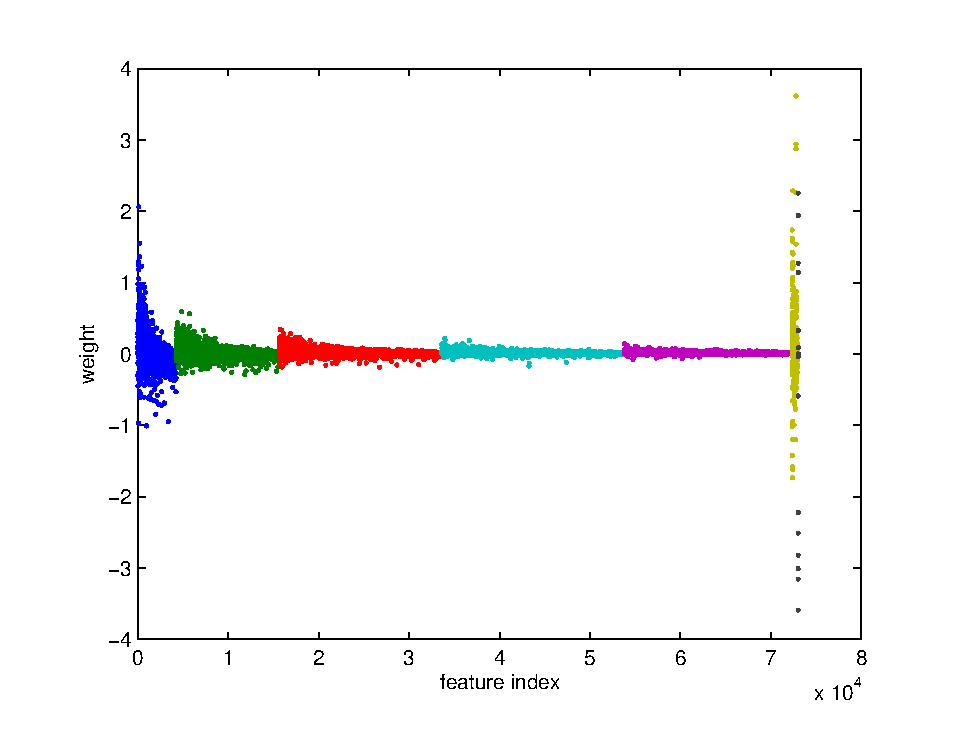
\includegraphics[width=7cm]{figures/SGDlambda}
\end{minipage}
\caption{Convergence of SGD for various values of $\lambda$. The green curve ($\lambda =10^{-3}$) represents the optimal value found by grid search. Higher values were also tried, but failed to converge for $\lambda > 10^{-3}$.}
\label{Fig:SGDlambda}
\end{figure}



As with the Viterbi algorithm, the forwards-backwards algorithm iteratively calculates tables of values for $\alpha(\cdot,\cdot)$. Features occuring at the beginning and end of labels were used to initialize the forwards and backwards tables.

Two methods were used to check the correctness of the forwards-backwards implementation. The partition function and log likelihood were computed combinatorically for a small test word for all possible labels. This was found to be numerically equal to the equivalent results generated by the forwards-backwards algorithm. Also, after training $\w$ by SGD, it was found that
\begin{equation}
\sum_{(\xb,\yb)\in T} Fj(\xb,\yb) \approx \sum_{(\x,\cdot)\in T} \mathbb{E}_{\y�\,|\,\x} \left[ F_j(\x, \y' ) \right]
\end{equation}
as predicted for the maximum $LCL$. Finally, gradients were checked agains their


\subsection{Design of Collins Perceptron}

The learning rate $\alpha$ was set to $0.02/T$. This is a widely used learning rate for gradient descent. Since Collins Perceptron is similar to gradient descent, this learning rate seemed appropriate.
The algorithm needs only 3 epochs until convergence in our case.

\subsection{Evaluation}
%Remember to put in real numbers here
Five-fold cross validation was used to evaluate the performance of our algorithm.  In each case, 7914 words were used to optimize parameter settings and train the feature weights. The remaining 1979 words were then used to test the accuracy of the trained classifier.

Two metrics were used to measure the accuracy of a prediction. For each test example, the Viterbi algorithm is used to predict a label, $\hat{y}_n$. The label is then compared to the true label, $y_n$, according to
\begin{enumerate}

\item Word Accuracy.
    \begin{equation}

\frac{\sum_{n=1}^N I(\hat{y}_n = y_n)}{N}

\end{equation}

\item Tag Accuracy

\begin{equation}

\frac{\sum_{n=1}^N \sum_{i=1}^{M_n} I(\hat{y}_{n,i} = y_{n,i})}{\sum_{n=1}^N M_n}.

\end{equation}
\end{enumerate}


\section{Results}
To test the algorithms the accuracy was measured using a 4-fold cross validation. The average word accuracy was about 74\%. The letter level accuracy was about 96\%. The results can be seen in Table \ref{result}.


\begin{table}
    \begin{tabular}{|l|l|l|}
    \hline
~&    Weight    & Feature
\hline
1&     3.6157    & Ends with a/0
2&   -3.5913    & VC/10
3&   -3.1576    & VC/01
4&   -3.0107
5&    2.9385
6&    2.8764
7&   -2.8241
8&   -2.5115
9&    2.2844
10&   2.2588
72789   pos(-1) a 04
73028   VC10
73027   VC01
73024   CV10
72791   pos(-1) e 04
72790   pos(-1) i 04
73020   CC10
73023   CV01
72419   pos(2) ng 01
72792   pos(-1) o 04

    \end{tabular}
    \caption{The top ten strongest weighted features. (Fold 2)
    \label{Tab:top10weights}
\end{table}

\begin{table}
    \begin{tabular}{|l|l|l|}
       \hline
       ~       & Word Level Accuracy & Letter Level Accuracy \\
       Test 1  & 0.70  &               0.95    \\
       Test 2  & 0.80    &             0.97                 \\
       Test 3  & 0.70           &             0.95                   \\
       Test 4  & 0.77    &             0.96                   \\
       Overall & 0.74                   &             0.96                   \\
       \hline
    \end{tabular}We change it to a four fold cross validation;)
    \caption{Results using Collins Perceptron with the Viterbi algorithm}
\label{results}
\end{table}

\section{Discussion}
\section{Conclusion}

Conditional Random Fields form a very general method for supervised learning. Their main strength comes from the huge variety of feature functions that can be used for analysis, and the fact that these features can be applied to non-numerical data such as natural languages.

In this study we were able to predict syllable boundaries with high accuracy. This can be attributed to our wide range of features, including both naive but comprehensive window features and more sophisticated consonant-vowel features based on prior linguistic knowledge.

\nocite{bishop06,bottou11,elkan11}
{\small
\bibliographystyle{ieee}
\bibliography{egbib}
}
\end{document}
